% \documentclass[german,bachelor,ul]{webisthesis} % Weimar
% \documentclass[german,bachelor,fsu]{webisthesis} % Jena
\documentclass[english,bachelor,ul]{webisthesis} % Leipzig
%
% Non-default programme
% ---------------------
% \documentclass[english,master,buw]{webisthesis}\global\thesisprogramme{Human-Computer Interaction}
% \documentclass[english,master,buw]{webisthesis}\global\thesisfrontpagefaculty{Faculty of Civil Engineering/Faculty of Media}\global\thesisprogramme{Digital Engineering}
% \documentclass[german,bachelor,buw]{webisthesis}\global\thesisprogramme{Informatik\\Schwerpunkt Medieninformatik}
% \documentclass[german,bachelor,buw]{webisthesis}\global\thesisprogramme{Informatik\\Schwerpunkt Security and Data Science}
%
% When you change the language, pdflatex may halt on recompilation.
% Just hit enter to continue and recompile again. This should fix it.


%
% Values
% ------
\ThesisSetTitle{Active Learning for Text Classification using Dimensionality Reduction for Core-Set}
\ThesisSetKeywords{Active Learning, Text Classification, Dimensionality Reduction, Core-Set, t-SNE} % only for PDF meta attributes
\ThesisSetLocation{Leipzig} 

\ThesisSetAuthor{Yannick Brenning}
\ThesisSetStudentNumber{3732848}
\ThesisSetDateOfBirth{27}{8}{2002}
\ThesisSetPlaceOfBirth{Bamberg}

% Supervisors should usually be Professors from the candidate's university. A second supervisor is not always needed. 
\ThesisSetSupervisors{Christopher Schröder, Christian Kahmann}

\ThesisSetSubmissionDate{31}{2}{2022}

%
% Suggested Packages
% ------------------
\usepackage[sort&compress]{natbib}
%   Allows citing in different ways (e.g., only the authors if you use the
%   citation again within a short time).
%
\usepackage{booktabs}
%    For tables ``looking the right way''.
%
% \usepackage{tabularx}
%    Enables tables with columns that automatically fill the page width.
%
% \usepackage[ruled,algochapter]{algorithm2e}
%    A package for pseudo code algorithms.
%
% \usepackage{amsmath}
%    For tabular-style formatting of mathematical environments.
%

\usepackage{fontawesome}
%    For lots of awesome glyphs: https://mirror.physik.tu-berlin.de/pub/CTAN/fonts/fontawesome/doc/fontawesome.pdf

\usepackage{multirow}
\usepackage{pdfpages}
\usepackage{graphicx}

%
% Commenting (by your supervisor)
% -------------------------------
\usepackage{xcolor}
\usepackage{soul}
\newcommand{\bscom}[2]{%
  % #1 Original text.
  % #2 Replacement text.
    \st{\scriptsize\,#1}{\color{blue}\scriptsize\,#2}%
  }

% Create links in the pdf document
% Hyperref has some incompatibilities with other packages
% Some other packages must be loaded before, some after hyperref
% Additional options to the hyperref package can be provided in the braces [], like in
% \usehyperref[backref] % This will add back references in the bibliography that some people like ... some don't ... so better ask your supervisor ;-)
\usehyperref

\begin{document}
\begin{frontmatter}
\begin{abstract}
This is the \LaTeX{} template for Bachelor and Master theses at Webis. This template contains several hints and conventions on how to structure a thesis, how to cite the work of others, and how to display your results besides plain text. 
\end{abstract}
\end{frontmatter}

\tableofcontents

\chapter{Introduction}

Text is one of the most widespread and important sources of information, but extracting data and tangible knowledge from it can be a difficult and expensive task. With the advent of the digital age, enormous amounts of unstructured texts are available with more being generated by the day. Due to this increasingly large amount of textual data, manually processing information at a larger scale becomes infeasible and thus demands the use of computer-driven approaches. 

The classification of text, meaning the assignment of a category or class to a document or piece of text is one of the most common and useful ways to gain information from a piece of text. As the amount of available text content continues to grow, text classification tasks become an increasingly important area of research within the field of natural language processing. 

Thanks to machine learning and data science, we have been able to develop many methods of extracting information from text, and as a result, perform text classification at a larger scale. This possibility for automated organization of data can enhance insights and decision-making across industries such as healthcare, finance, and social sciences, among many others. Active Learning (AL) is a subfield of machine learning in which the learning algorithm is able to perform queries on an information source in order to reduce the total amount of annotated data. This method can offer significant advantages in improving model performances and especially in reducing labeling costs. Though there is no universally good strategy, AL has been proven to be useful in many cases where annotating data is expensive or the total amount of data is very large (\cite{settles.tr09}). 

% One such model is the CNN (convolutional neural network), which is used in many recognition and learning tasks but needs to be trained on a large dataset. With AL, selecting the most effective data points to be labelled by the oracle from a large pool of unlabelled data can be a challenge, especially in the case of CNNs. 
Oftentimes, there is a large amount of unlabelled available data for an AL model to learn from. In this case, selecting the most effective data points to be labelled by the information source from this large pool becomes a crucial, but difficult challenge to overcome. 

One attempt at improving the effectiveness of AL in this regard is the Core-Set approach (\cite{DBLP:conf/iclr/SenerS18}) This method uses core-set selection to counter the issue of AL ineffectiveness on convolutional neural networks. The proposed approach selects a set of points the pool such that a model learning over this subset can be consistent when provided the remaining data points. The method was shown to have improved results when compared to other approaches in the field of computer vision (\cite{DBLP:conf/iclr/SenerS18}, \cite{DBLP:conf/cvpr/CaramalauBK21}), which encompasses tasks that focus on enabling computers to interpret and understand visual information from the world. This field involves a variety of different methods including image classification, object detection, and semantic segmentation, all of which have significant importance in scientific research, classification tasks, and pattern recognition.

However, Core-Set has been shown to have mixed results in cases of text classification using BERT (\cite{DBLP:conf/kdd/0002MM21}, \cite{DBLP:conf/emnlp/Ein-DorHGSDCDAK20}) and binary text classification using DNNs (\cite{DBLP:conf/cikm/Liu0LZW21}). Particularly in the first case, the experiments show that Core-Set performs poorly even when compared to the random sampling strategy. In addition, the approach has even been shown to be less effective in computer vision tasks in cases with higher numbers of classes as well as higher-dimensional data points (\cite{DBLP:conf/iccv/SinhaED19}). The theoretical analysis shown in \cite{DBLP:conf/iclr/SenerS18} briefly mentions this within the context of higher class amounts, however it does not attempt to provide a potential solution to the problem.

% Particularly in first case, the experiments conducted on the Internal Dataset and TREC-6 show that Core-Set performs poorly when comparing the F1-scores to the random sampling strategy. 

This thesis aims to explore the possibility of improving the Core-Set approach for text classification tasks. By first explaining Core-Set's functionality and the theoretical reasons for why it tends to underperform in certain classification tasks, I aim to then demonstrate the performance difference in comparison to various baseline approaches on large datasets of text content in order to verify this claim. Furthermore, this thesis looks to improve on the Core-Set approach within the context of text classification tasks and demonstrate this improvement as a part of its experiment.

In the following, Chapter 2 explains the background and related work on the topics of text classification (Section 2.1), active learning in general (Section 2.2), and the Core-Set approach to AL more specifically (Section 2.3). In Chapter 3, I will explain my approach to improving the performance of Core-Set for text classification using dimensionality reduction. In Chapters 4 and 5, I will present my experiment as well as discuss its results. Finally, Chapter 6 will conclude the thesis and provide insights on potential future developments of the method. 

\chapter{Background/Related Work}

\section{Text Classification}

% **GENERAL**
Text classification is one of the most fundamental and important tasks in the field of Natural Language Processing (NLP). As a result, developing efficient automatic text classification methods has become an important research topic. 

% **APPLICATION**
One of the most common applications of text classification is determining whether the opinion associated with a certain document has a positive or negative sentiment, also known as sentiment analysis. This has a wide range of uses, including the possibility for businesses to better gauge customer opinions on products and services (\cite{DBLP:books/sp/mining2012/LiuZ12}) in order to adapt accordingly. This application is a binary classification task, meaning the classifier has two classes with which each document can be labelled (positive or negative). Similarly, one might apply this binary classification task to the problem of spam filtering in e-mails, text messages and more. 

Beyond that, many applications of text classification require multiple classes, such as news and content categorization. In this case, text classification algorithms can organize documents into specific topics or themes (e.g. Sports, Business, Politics, \dots) (\cite{DBLP:journals/csur/Sebastiani02}). Other applications include information retrieval, recommender systems, and document summarization (\cite{DBLP:journals/information/KowsariMHMBB19}).

% **PROCESS**
Generally, text classification methods can be divided into the following phases: data collection and preprocessing, feature extraction, classifier selection, and model evaluation (\cite{DBLP:journals/information/KowsariMHMBB19}, \cite{DBLP:journals/eswa/MironczukP18}, \cite{ikonomakis2005text}).

In the first stage, some form of text data necessary to complete some classification objective is acquired, ideally of a sufficient amount. There are several open data sets that are publicly available for this stage. The preprocessing phase includes steps such as lemmatization, removal of stop words, tokenization and stemming. 

The preprocessed text data must them be converted into numerical feature vectors. There are a number of techniques for accomplishing this such as Bag-of-Words, TF-IDF (Term Frequency-Inverse Document Frequency), and word embedding methods such as Word2Vec or GloVe. In addition to the methods just mentioned which are known as static word embeddings, there exist context-sensitive methods as of the late-2010s such as BERT and ELMo (\cite{DBLP:conf/naacl/DevlinCLT19}, \cite{DBLP:conf/naacl/PetersNIGCLZ18}), which can better represent the varied senses encompassed by words depending on their contexts.

The next phase, classifier selection, is one of the most crucial steps in the text classification pipeline. Without a comprehensive grasp of the underlying concepts of each algorithm, we cannot effectively determine an appropriate model for the task. Commonly known algorithms include Logistic Regression, Naive Bayes and Support Vector Machines. More recently deep learning models such as Convolutional Neural Networks (CNNs), Recurrent Neural Networks (RNNs) and Transformer Models have become established as state-of-the-art approaches, especially when considering large text classification tasks. These different deep learning algorithms are increasingly popular due to their ability to model more complex and non-linear relationships within data (\cite{DBLP:journals/nature/LeCunBH15}). The Core-Set approach was also originally developed for the deep learning domain, more specifically CNNs. As a result, this thesis will also be focusing on the use of deep learning models, specifically transformers.

Model evaluation is usually the "final" phase of the text classification process. This encompassees the assessment of the classifier's performance, for which a myriad of metrics such as accuracy, F1-score and AUC can be employed. Based on the evaluation, one can select a suitable model/strategy as well as attempt to optimize it.

The process of text classification clearly includes many steps which can be optimized and examined. Due to this, going over the entire process in detail would exceed the scope of this thesis. With this in mind, this thesis' experiment does not focus on the initial steps such as data collection, preprocessing and feature extraction, but rather the model training and evaluation steps.

% **CHALLENGES(?)**

\section{Active Learning}

Active Learning has become an increasingly important field when considering the need for efficient models as well as the labelling bottleneck in various machine learning tasks. Many fields, such as speech recognition, information extraction and classification suffer from this bottleneck as a result of their instance labels being expensive or time-consuming to obtain (\cite{settles.tr09}). 

Generally, active learning takes place in one of three main scenarios, namely \textit{membership query synthesis}, \textit{stream-based selective sampling} and \textit{pool-based active learning}. 

In the case of membership query synthesis, a membership query is created in the form of some unlabelled instance from the original dataset (\cite{DBLP:journals/ml/Angluin87},\cite{DBLP:journals/ijon/WangHYL15}). In other words, this approach synthesizes a query de novo, rather than selecting some query from the instance space. One challenge of this approach is ensuring that the synthesized query is consistent with meeting the constraints imposed by the real data. In the case of a human oracle, this can result in unrecognizable queries, for example in the case of computer vision tasks. Similarly, this issue could also apply to text classification, where the query synthesis produces unintelligible texts (\cite{langbaum92}, \cite{settles.tr09}).% TODO: Can I cite two papers for "essentially" the same definition (first one is the original paper, second one's explanation seemed more clear)

Stream-based selective sampling, on the other hand, typically examines each unlabelled instance one at a time and decides whether to query the oracle or to assign a label (\cite{settles.tr09}).

Finally, we consider the pool-based approach as one of the commonly known applications of AL. This scenario assumes a large set of unlabelled instances and a small set of labelled instaces, from which queries can be selectively drawn using a \textit{query strategy}. This can be useful in many real-world problems where plenty of unlabelled data is available and the pool is assumed to be closed (though this is not necessarily always the case) (\cite{settles.tr09}).

This thesis considers the case of the pool-based scenario, as does the original Core-Set paper. It is worth mentioning however, that Core-Set has also been applied in the stream-based context (\cite{DBLP:conf/icml/SaranYK0A23}).

\section{Core-Set}

The Core-Set approach as proposed in \cite{DBLP:conf/iclr/SenerS18} was originally designed for convolutional neural networks (CNNs) to tackle the problem of AL algorithms on large datasets. The empirical studies conducted by \cite{DBLP:conf/iclr/SenerS18} show that Core-Set outperforms other approaches within the field of image classification.

The task of active learning is defined as a \textit{core-set selection} problem in which the algorithm selects a smaller subset of points with increased diversity to learn from such that the model can be competitive over a larger dataset. This problem ends up being equivalent to the \textit{k-Center} problem (\cite{DBLP:conf/iclr/SenerS18}), which is also referred to as the minimax facility location problem. 

In mathemetical terms, given a set of points $ N $ and a budget $ k \leq |N| $, k-Center finds a subset $ \mathbf{s} \subseteq N $ of $ k $ points such that the minimum distance of any point in $ N \setminus \mathbf{s} $ to its closest center in $ \mathbf{s} $ is maximal. Another way of viewing this problem is by placing circles around the points in our set of centers. If we denote the maximum distance of any point in $ N $ to its nearest center in $ \mathbf{s} $ with $ \delta_{\mathbf{s}} $ and we place circles with a $ \delta_{\mathbf{s}} $-radius around each center in $ \mathbf{s} $, we can "cover" the entire set of points $ N $. In other words, k-Center attempts to find the minimum $ \delta_{\mathbf{s}} $ such that all points lie within the union of the $ \delta_{\mathbf{s}} $-circles when placed upon each center. This problem has been shown to be NP-hard (\cite{DBLP:journals/dam/HsuN79}, \cite{DBLP:journals/anor/Hochbaum84}). As a result, Core-Set uses a greedy approach to solve the Core-Set problem. However, it is worth noting that approximations of the algorithm are bound by twice the optimal solution (\cite{DBLP:journals/dam/HsuN79}). 

Let $ OPT $ denote the maximum distance of a center to a point in the optimal solution to k-Center. Then k-Center greedy's resulting maximum distance $ \delta_{\mathbf{s}} $ to any center in $ \mathbf{s} $ is at the worst $ 2 \cdot OPT $. The original paper by Sener and Saverese attempts to further improve the robustness of this approximation by placing an upper limit on the number of outliers that can be selected. This thesis will be focusing on and using the regular k-Center greedy algorithm for ease of implementation and interpretability. (?)

\section{Dimensionality Reduction}

As mentioned earlier, one of the major challenges of the Core-Set approach (among others) is handling data points with a higher dimensionality (\cite{DBLP:conf/iccv/SinhaED19}). Broadly speaking, this is a phenomenon coined by Richard E. Bellman known as the \textit{curse of dimensionality} (\cite{franccois2007high}). As a result, many algorithms have been developed to transform data from a high-dimensional space into a low-dimensional space. This task directly poses another challenge: managing to reduce the dimensionality of the data while still being able to retain the highest possible amount of information. 

One such method is the Principal Components Analysis (PCA), which is one of the most popular linear techniques for dimensionality reduction (\cite{van2009dimensionality}). In essence, PCA linearly transforms the data into a representation that attempts to closely describe the variance of the initial data (\cite{jolliffe2016principal}). Other commonly used linear techniques include Linear Discriminant Analysis (LDA), Multidimensional Scaling (MDS), and Non-negative Matrix Factorization (NMF).

These techniques can be powerful, however they often miss important non-linear structures in high-dimensional data. Therefore, non-linear techniques have been developed such as Isometric Mapping (Isomap) and t-distributed Stochastic Neighbor Embedding (t-SNE). The latter is a relatively modern probablistic approach that has improved upon many other non-linear techniques in creating a single map that reveals structure on many different scales. In addition, it manages to reduce the tendency of SNE to crowd data points together at the center by using a different cost function (\cite{van2008visualizing}). 

First, it converts the high-dimensional Euclidean distances into conditional probabilities, such that similar data points are assigned higher probabilities and dissimilar data points are assigned very low probabilities. It then creates a similar probability distribution over the lower-dimensional map such that the \textit{Kullback-Leibler divergence} (a measure of how one probability distribution differs from another) is minimized.

This method is especially useful for the visualization of high-dimensional data, in which the aim is to display and view the underlying structure in a given dataset. t-SNE plots are strongly influenced by the chosen hyperparameters however, and thus a good understanding for the influence of these parameters is important. Particularly \textit{perplexity}, a measure of the effective number of neighbours, has a complex effect on the resulting reductions. According to \cite{van2008visualizing}, typical values for perplexity are between 5 and 50 and larger/denser datasets often generally require higher perplexities (\cite{vanHomepage}). Other commonly adjusted parameters include the learning rate and number of iterations for the optimization.

\chapter{Approach}

As mentioned, distance-based methods such as Core-Set can be ineffective in higher dimensions. To overcome this challenge, I propose the application of t-SNE as a dimensionality reduction technique on the training data before employing the Greedy Core-Set strategy. In order to optimize my use of t-SNE, I will first examine the effects of different hyperparameters on the reductions. Based on these examinations, I will select the optimal t-SNE parameters to use for the experiment. 

Next, I will examine the effect of pointwise probabilities on the Core-Set algorithm. Core-Set currently operates using the distances between its points -- in this experiment, I propose an approach where Core-Set considers the probability distributions in addition to the distances. 

To accomplish this, I will be using an uncertainty-based approach. Uncertainty sampling, which was introduced by \cite{DBLP:conf/sigir/LewisG94}, essentially attempts to select the unlabelled examples with the lowest classification certainty. In this case, I specifically opted for an approach similar to that of Breaking-Ties (\cite{DBLP:journals/jmlr/LuoKGHSRH05}), where the instances with the smallest margin between their top two most likely classification probabilities are selected, essentially "breaking the tie" between the two most likely classes. The results of this calculation will then be multiplied as a weight vector with the distances normally used by Core-Set.

This approach resulted in two different implementation ideas: the first, which we will call "Weighted Greedy Core-Set" (WCS), calculates the uncertainties prior to executing the standard Core-Set algorithm, then multiplies the resulting Core-Set distances and probabilities using weights (in this case, I used a 80-20 weighting in favour of the Core-Set distances). 

The second, which I will call "Ranked Weighted Greedy Core-Set" (RWCS), opts to first compute a Core-Set twice the size of the original sample size $n$, then "re-ranks" the resulting distances according to Breaking-Ties uncertainties and finally selects the points with the $n$ highest uncertainties.

Finally, I will take into account the class distributions within each Core-Set and select points based on the representation of each class.

The experiment will be conducted with two models on three well-known classification datasets and will measure the performances throughout 5 runs per combination. I have chosen two state-of-the-art transformers, BERT (\cite{DBLP:conf/naacl/DevlinCLT19}) and SetFit (\cite{DBLP:setfit}) as models for this experiment.

\chapter{Experiment}

\section{Data}

This experiment was conducted across three datasets commonly used in the field of AL. These datasets are of three different types: sentiment analysis (S), questions (Q), and news (N). For binary classification, I used \textbf{Movie Review}, a sentiment analysis dataset (\cite{DBLP:conf/acl/PangL05}) containing 5,331 positive and 5,331 negative samples. For multi-class text classification, \textbf{AG's News} (\cite{DBLP:conf/nips/ZhangZL15}), comprised of 120,000 training samples and 7,600 test samples, and \textbf{TREC} (\cite{DBLP:journals/nle/LiR06}), a question dataset containing 5,500 training samples and 500 test samples.

The test set was only provided in the case of AG's News and TREC, in the case of Movie Review I employed a split of the 10,662 samples myself. \dots

% The chosen datasets are Movie Review (MR), a sentiment analysis dataset with 10662 data points, TREC-6, a question dataset with {} data points, and finally AG-News, a topic dataset with 120,000 data points. Each of these datasets is commonly used in the field of AL. One must note that these are comparatively few data points, due to the fact that AL is a time and resource-expensive field.

\section{Experiment Setup}

As mentioned earlier, setting t-SNE's hyperparameters and exploring the resulting differing reduction behaviours has been shown to often be necessary (\cite{wattenberg2016how}). \cite{vanHomepage} mentions that examining the resulting plots is one of the best ways to assess the quality of the visualizations, in addition to comparing the Kullback-Leibler divergences. 

Below, I have demonstrated the effect of t-SNE on a training set of the MR dataset (\cite{DBLP:conf/acl/PangL05}) containing 9,596 samples with a feature dimension of 768. The reductions are completed using perplexity values of 5, 30, 50 and 100 with iteration counts of 1,000 and 5,000 respectively. Note that the samples have been embedded using BERT and then normalized prior to the dimensionality reductions.

\iffalse
\begin{figure}[htbp]
    \centering
    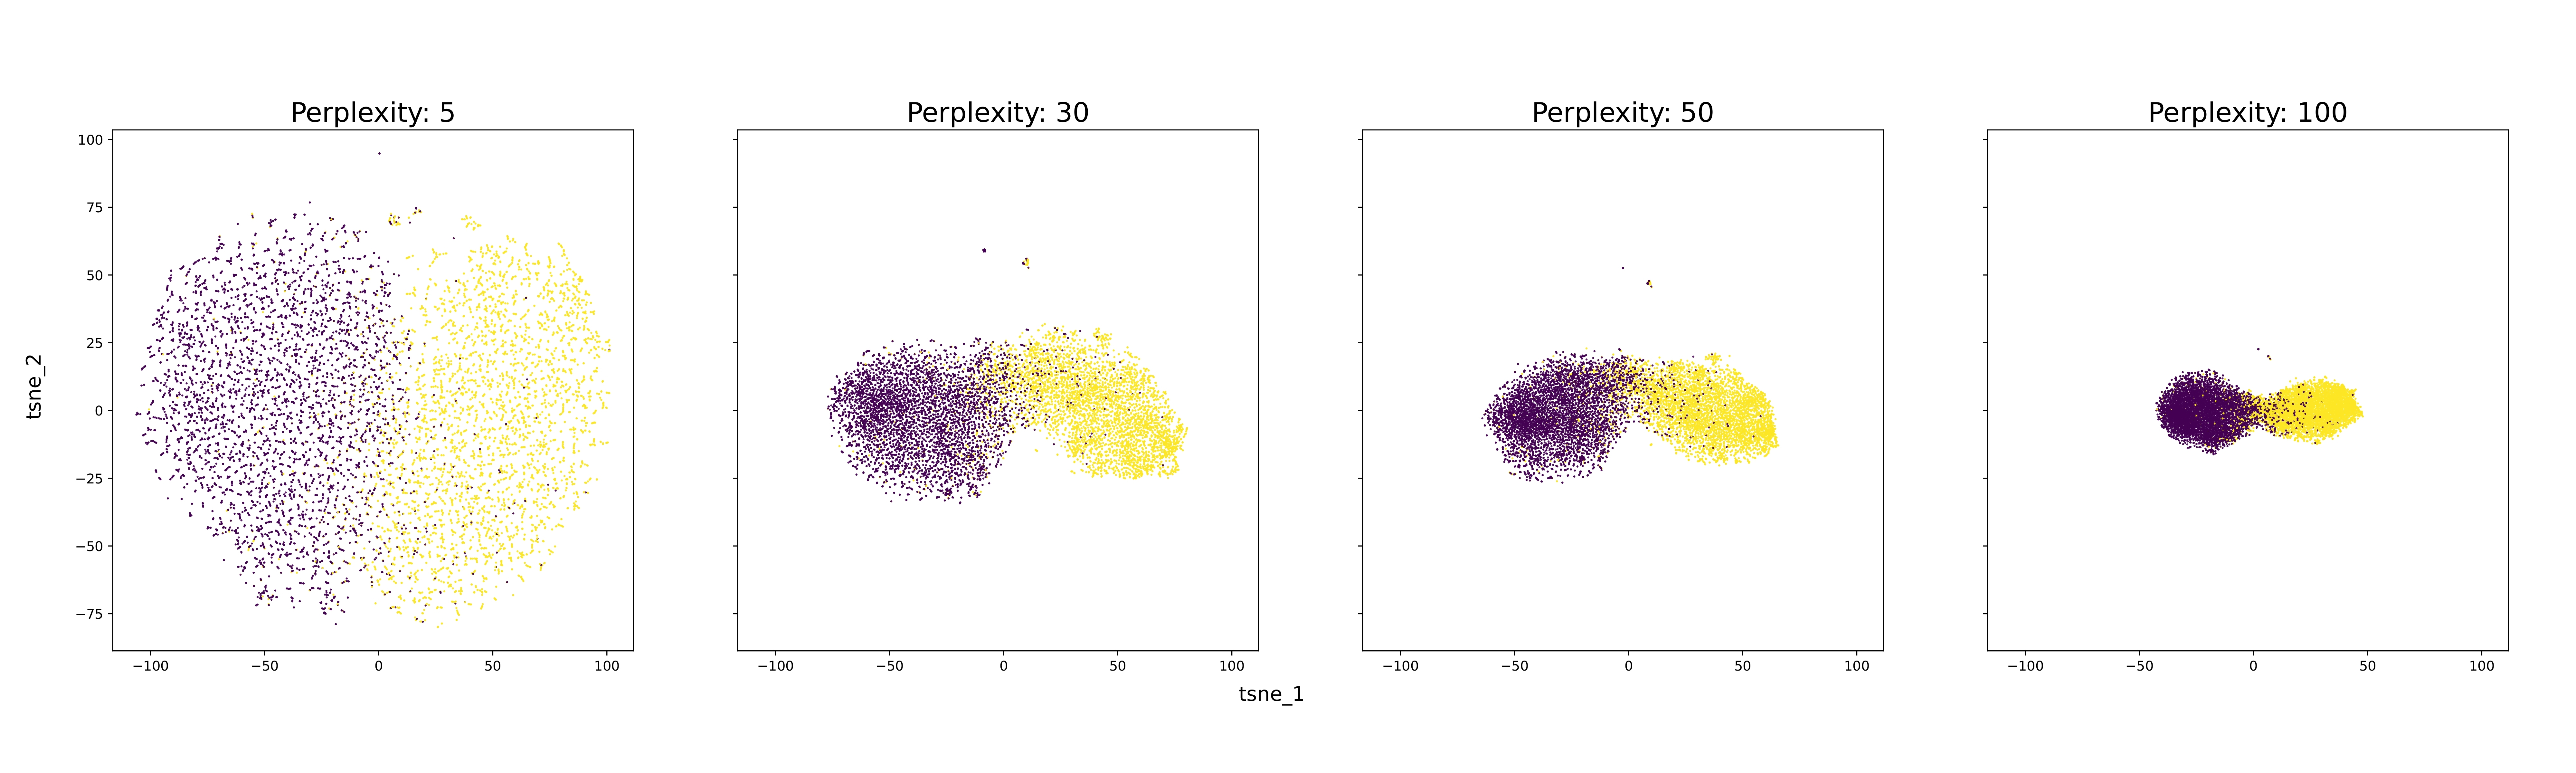
\includegraphics[width=1\textwidth]{img/reductions-mr-1000.jpg}
    \caption{t-SNE reductions with various perplexity values after 1,000 iterations performed on the embedded and normalized Movie Review dataset.}
    \label{fig:reductions-mr-1000}
\end{figure}

\begin{figure}[htbp]
    \centering
    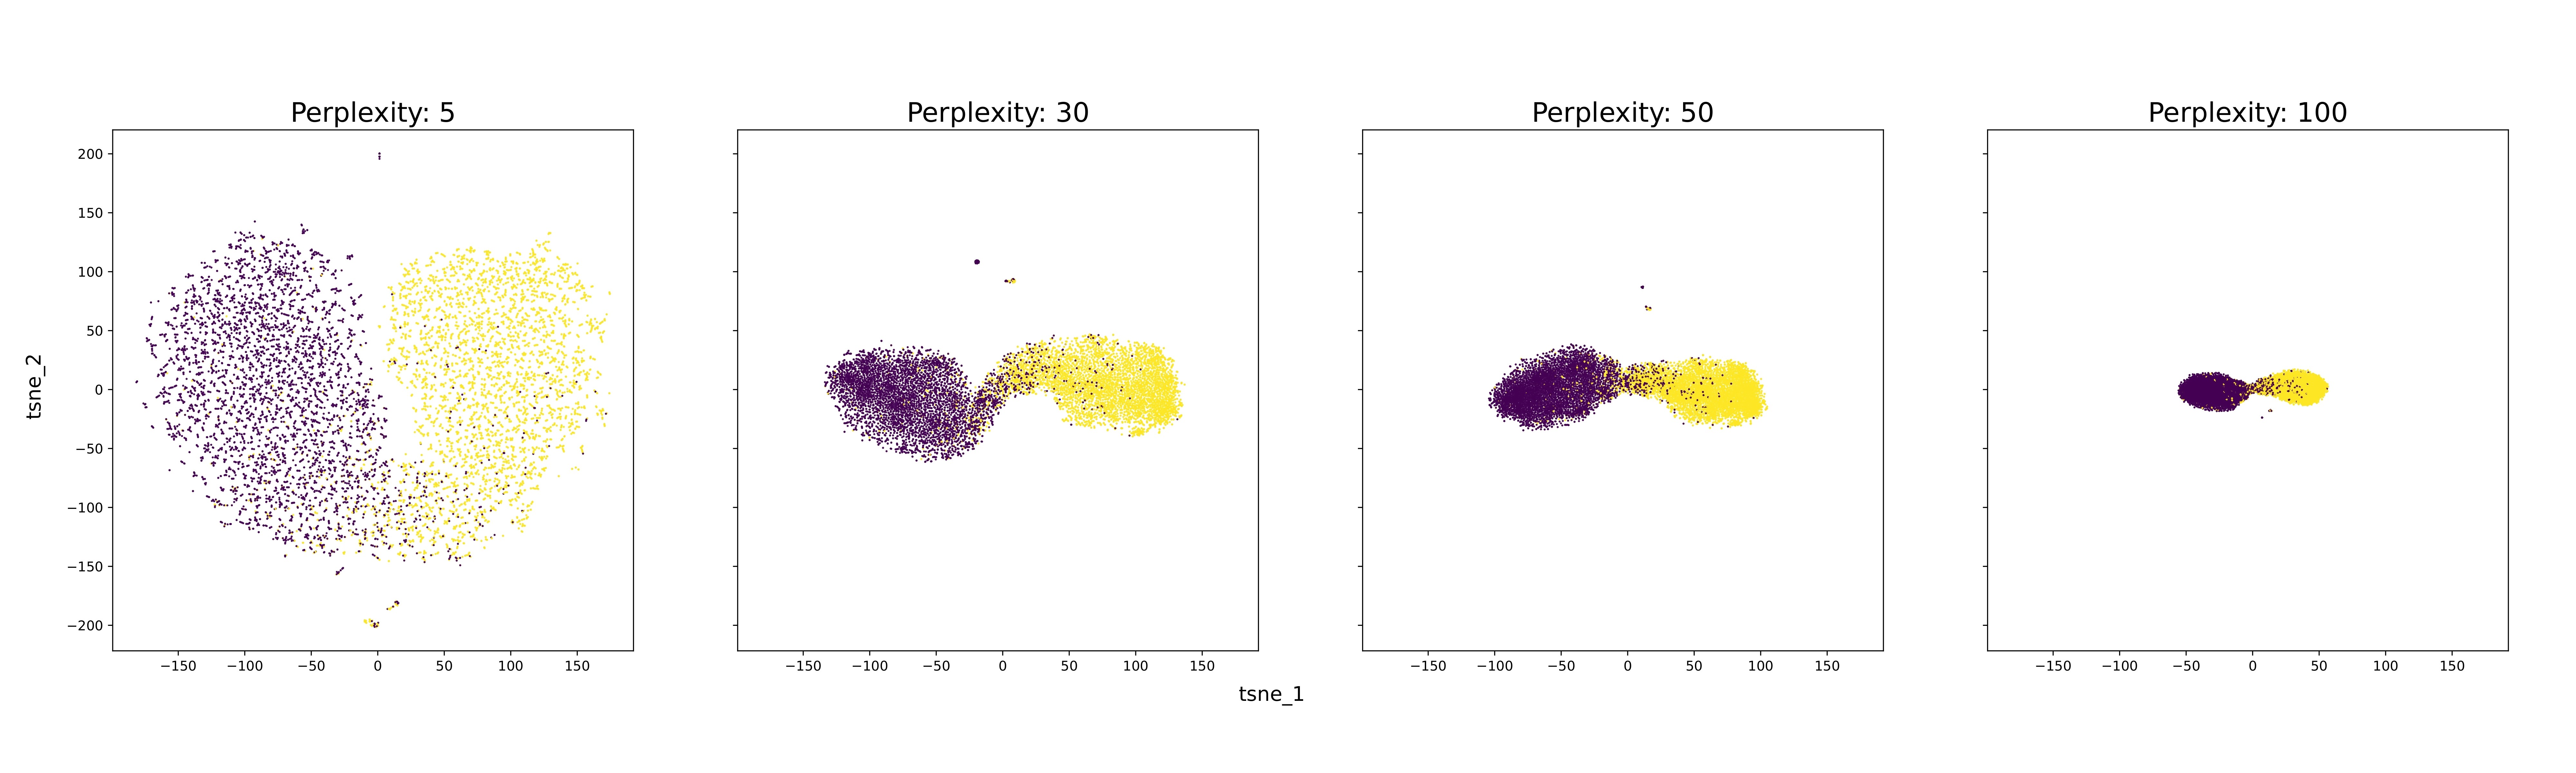
\includegraphics[width=1\textwidth]{img/reductions-mr-5000.jpg}
    \caption{t-SNE reductions with various perplexity values after 5,000 iterations performed on the embedded and normalized Movie Review dataset.}
    \label{fig:reductions-mr-5000}
\end{figure}

\begin{figure}[htbp]
    \centering
    \includegraphics[width=1\textwidth]{img/reductions-ag-news-1000.jpg}
    \caption{t-SNE reductions with various perplexity values after 1,000 iterations performed on the embedded and normalized AG's News dataset.}
    \label{fig:reductions-agnews-1000}
\end{figure}

\begin{figure}[htbp]
    \centering
    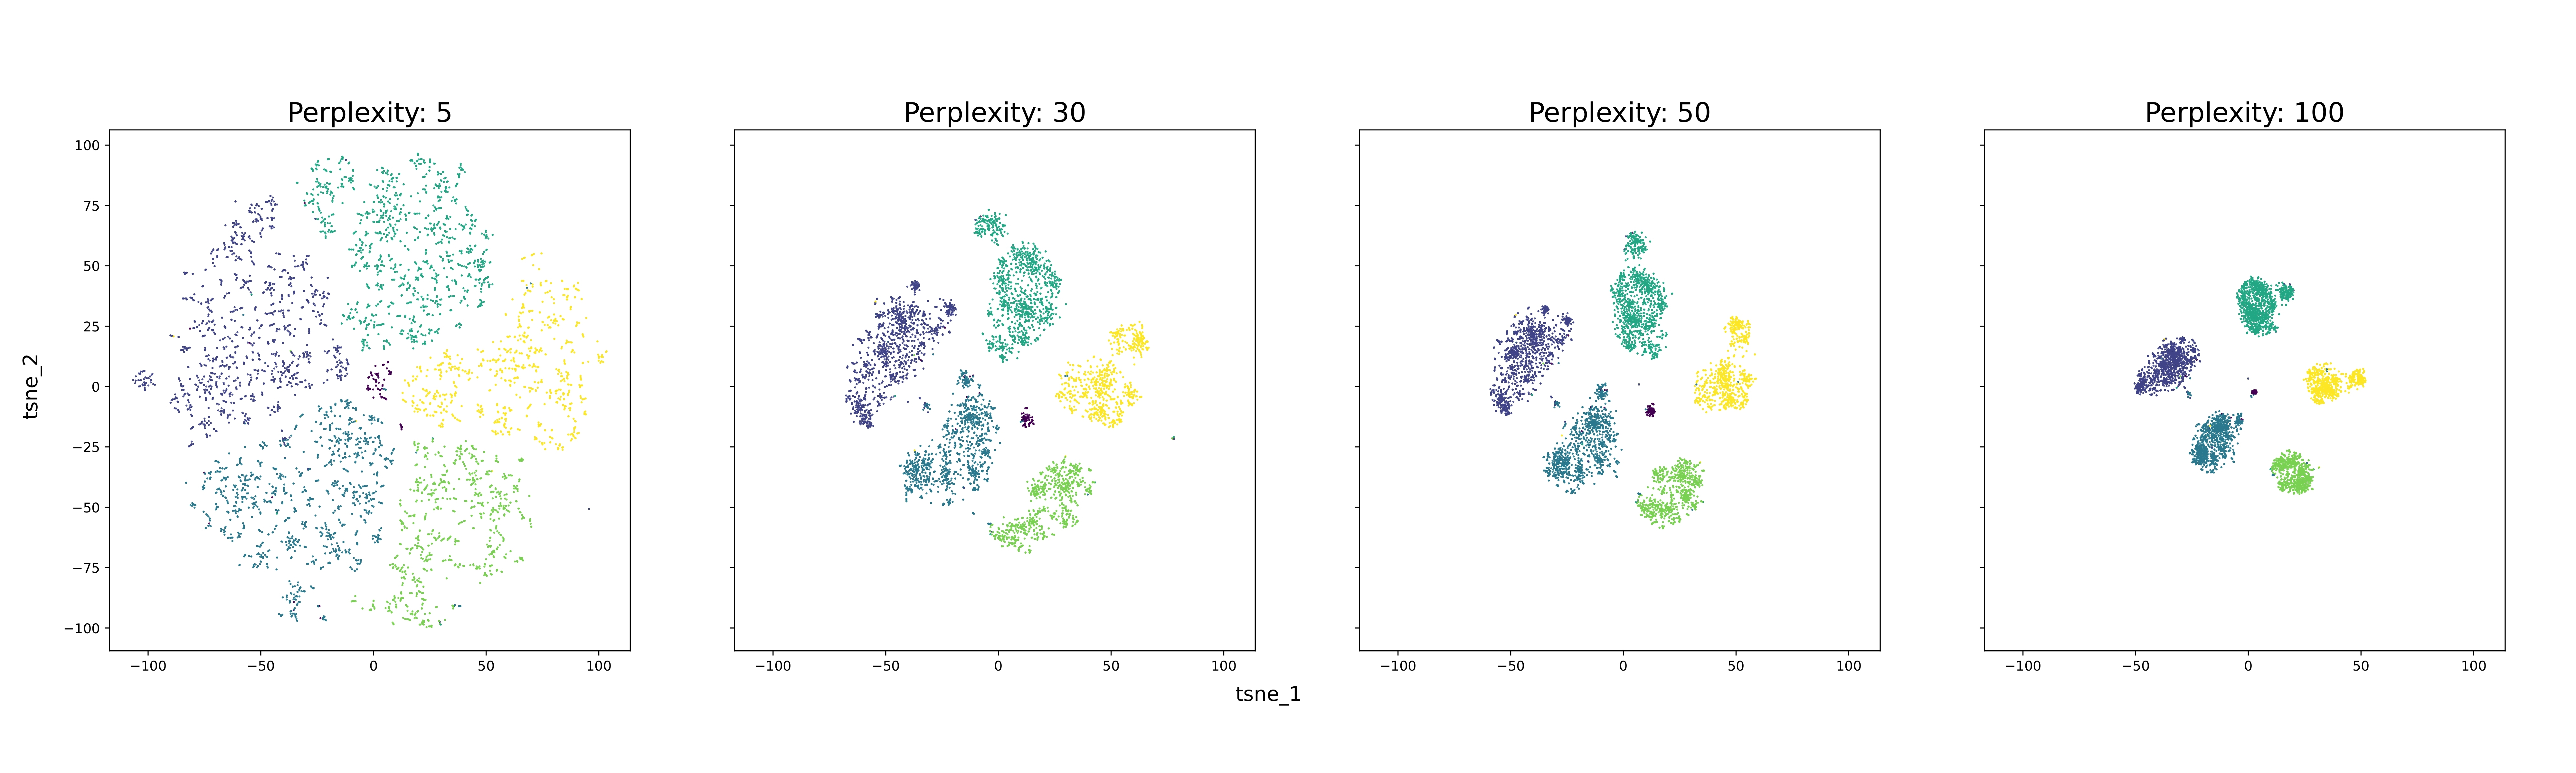
\includegraphics[width=1\textwidth]{img/reductions-trec-1000.jpg}
    \caption{t-SNE reductions with various perplexity values after 1,000 iterations performed on the embedded and normalized TREC-6 dataset.}
    \label{fig:reductions-trec-1000}
\end{figure}

\fi

Starting at a perplexity of 30, the points begin to cluster more and more tightly. The clusters do not seem to separate in any of the runs -- it is important to note, however, that distances and sizes of the clusters do necessarily carry any meaning when examining the reduction plots (\cite{wattenberg2016how}, \cite{vanHomepage}).

It is also worth noting that the differences between 1,000 and 5,000 iterations appear quite small despite the relative increase in computations. \dots

The experiment is conducted using 20 queries on 25 instances, with a validation set size of 10\%. The experiment is averaged over five runs of queries per combination of dataset, model and query strategy. 

\section{Experiment Results}

The following figures show the learning curves for each combination of dataset, model and query strategy. 

\begin{figure}[htbp]
    \centering
    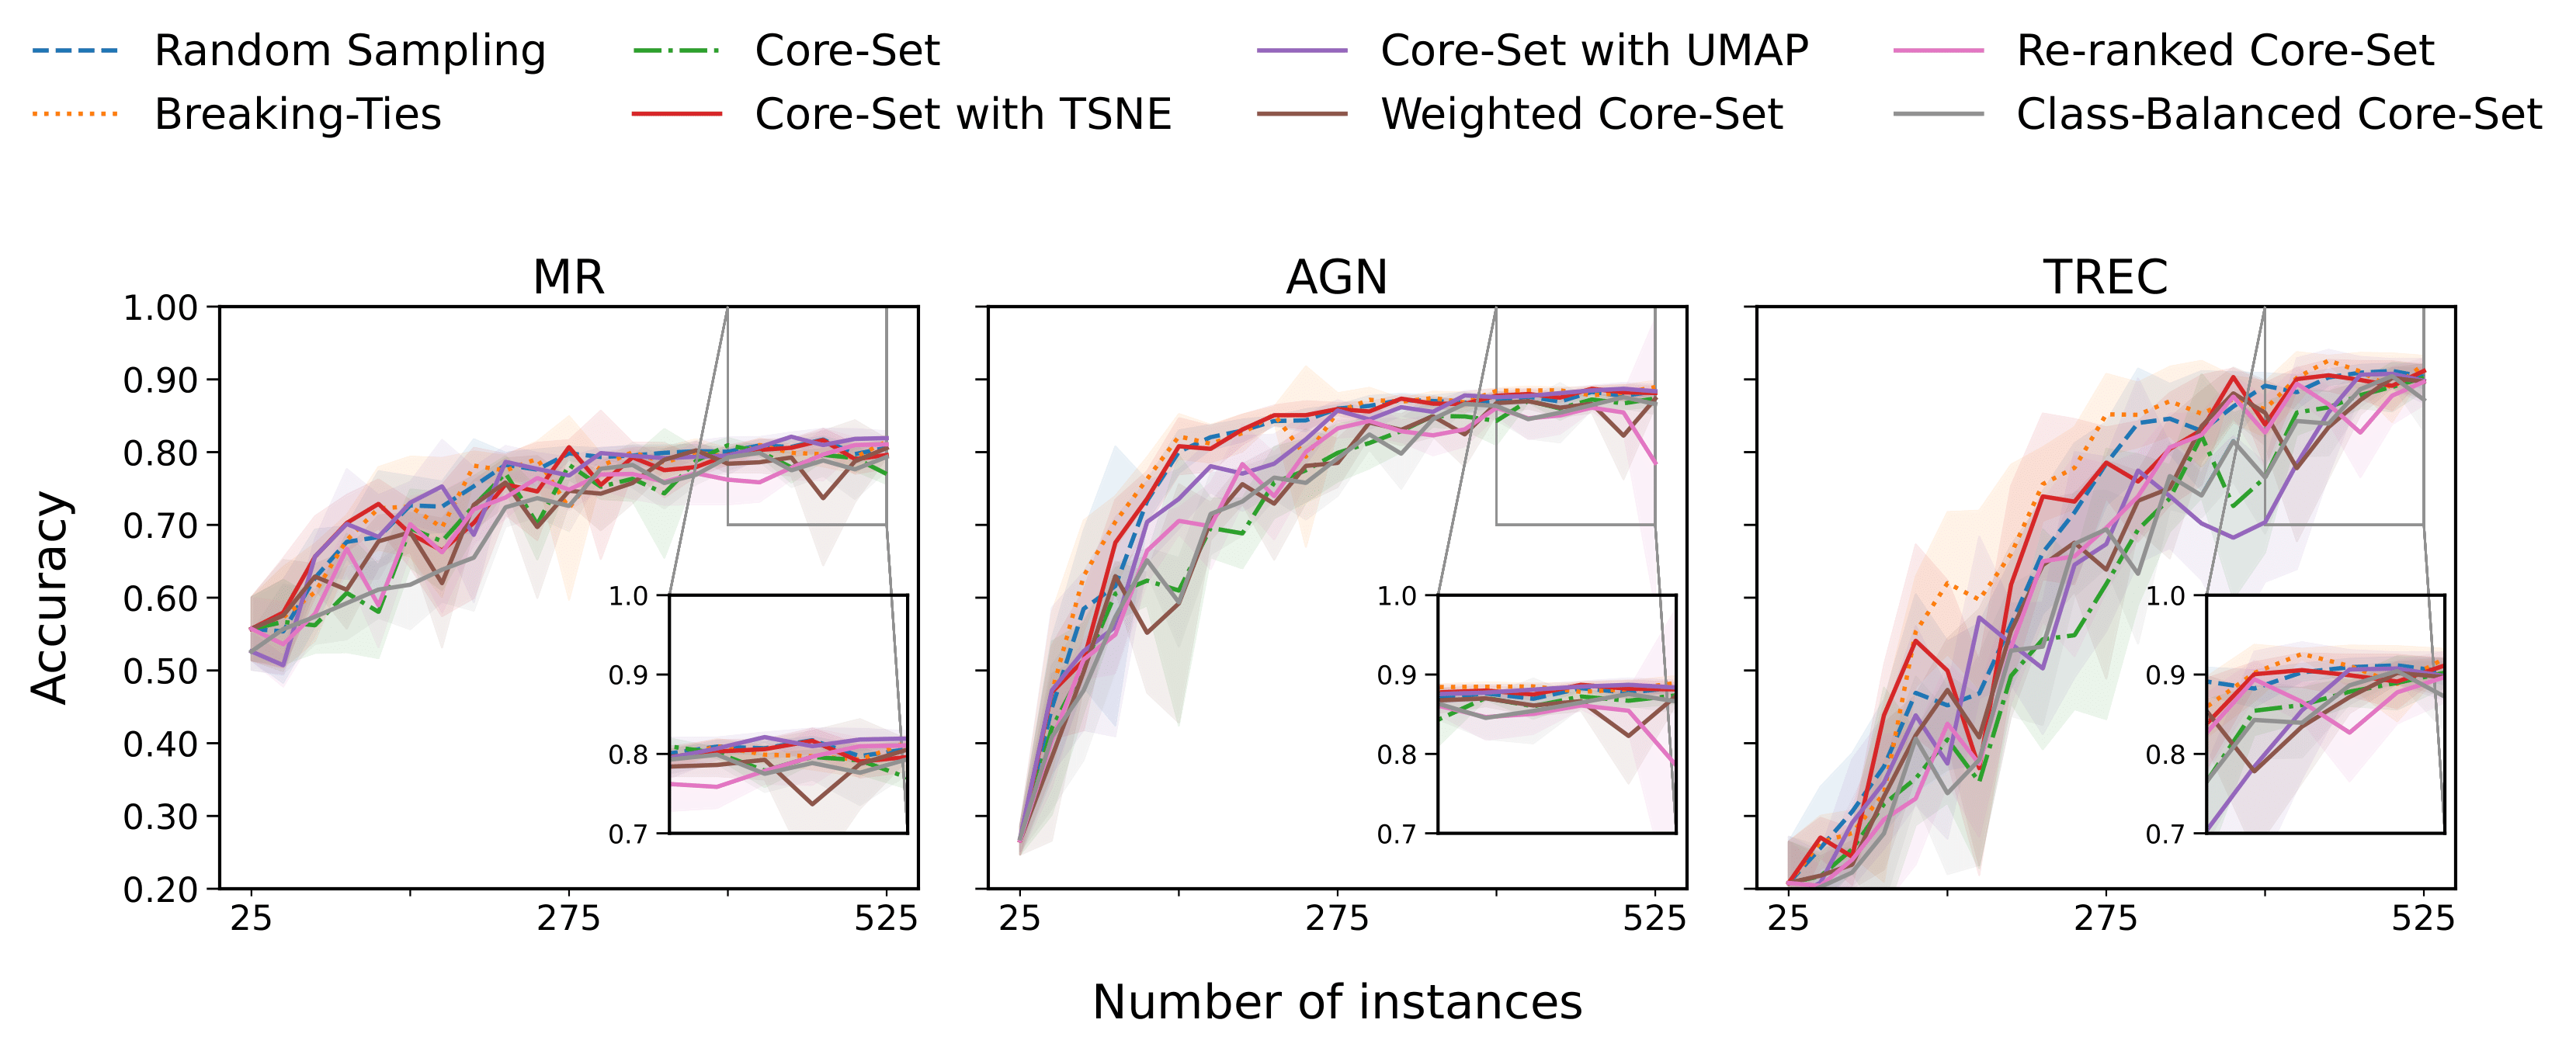
\includegraphics[width=1\textwidth]{img/bert-plots-1.png}
    \caption{Active Learning curves of BERT on each dataset when combined with six query strategies: Random Sampling (RS), Breaking-Ties (BT), Greedy Core-Set (CS), Greedy Core-Set with t-SNE (CS-TSNE), Weighted Greedy Core-Set (WCS), and Ranked Weighted Greedy Core-Set (RWCS). The line represents the mean accuracy and the surrounding tubes represent the standard deviation over five runs.}
    \label{fig:bert-curves}
\end{figure}

\begin{figure}[htbp]
    \centering
    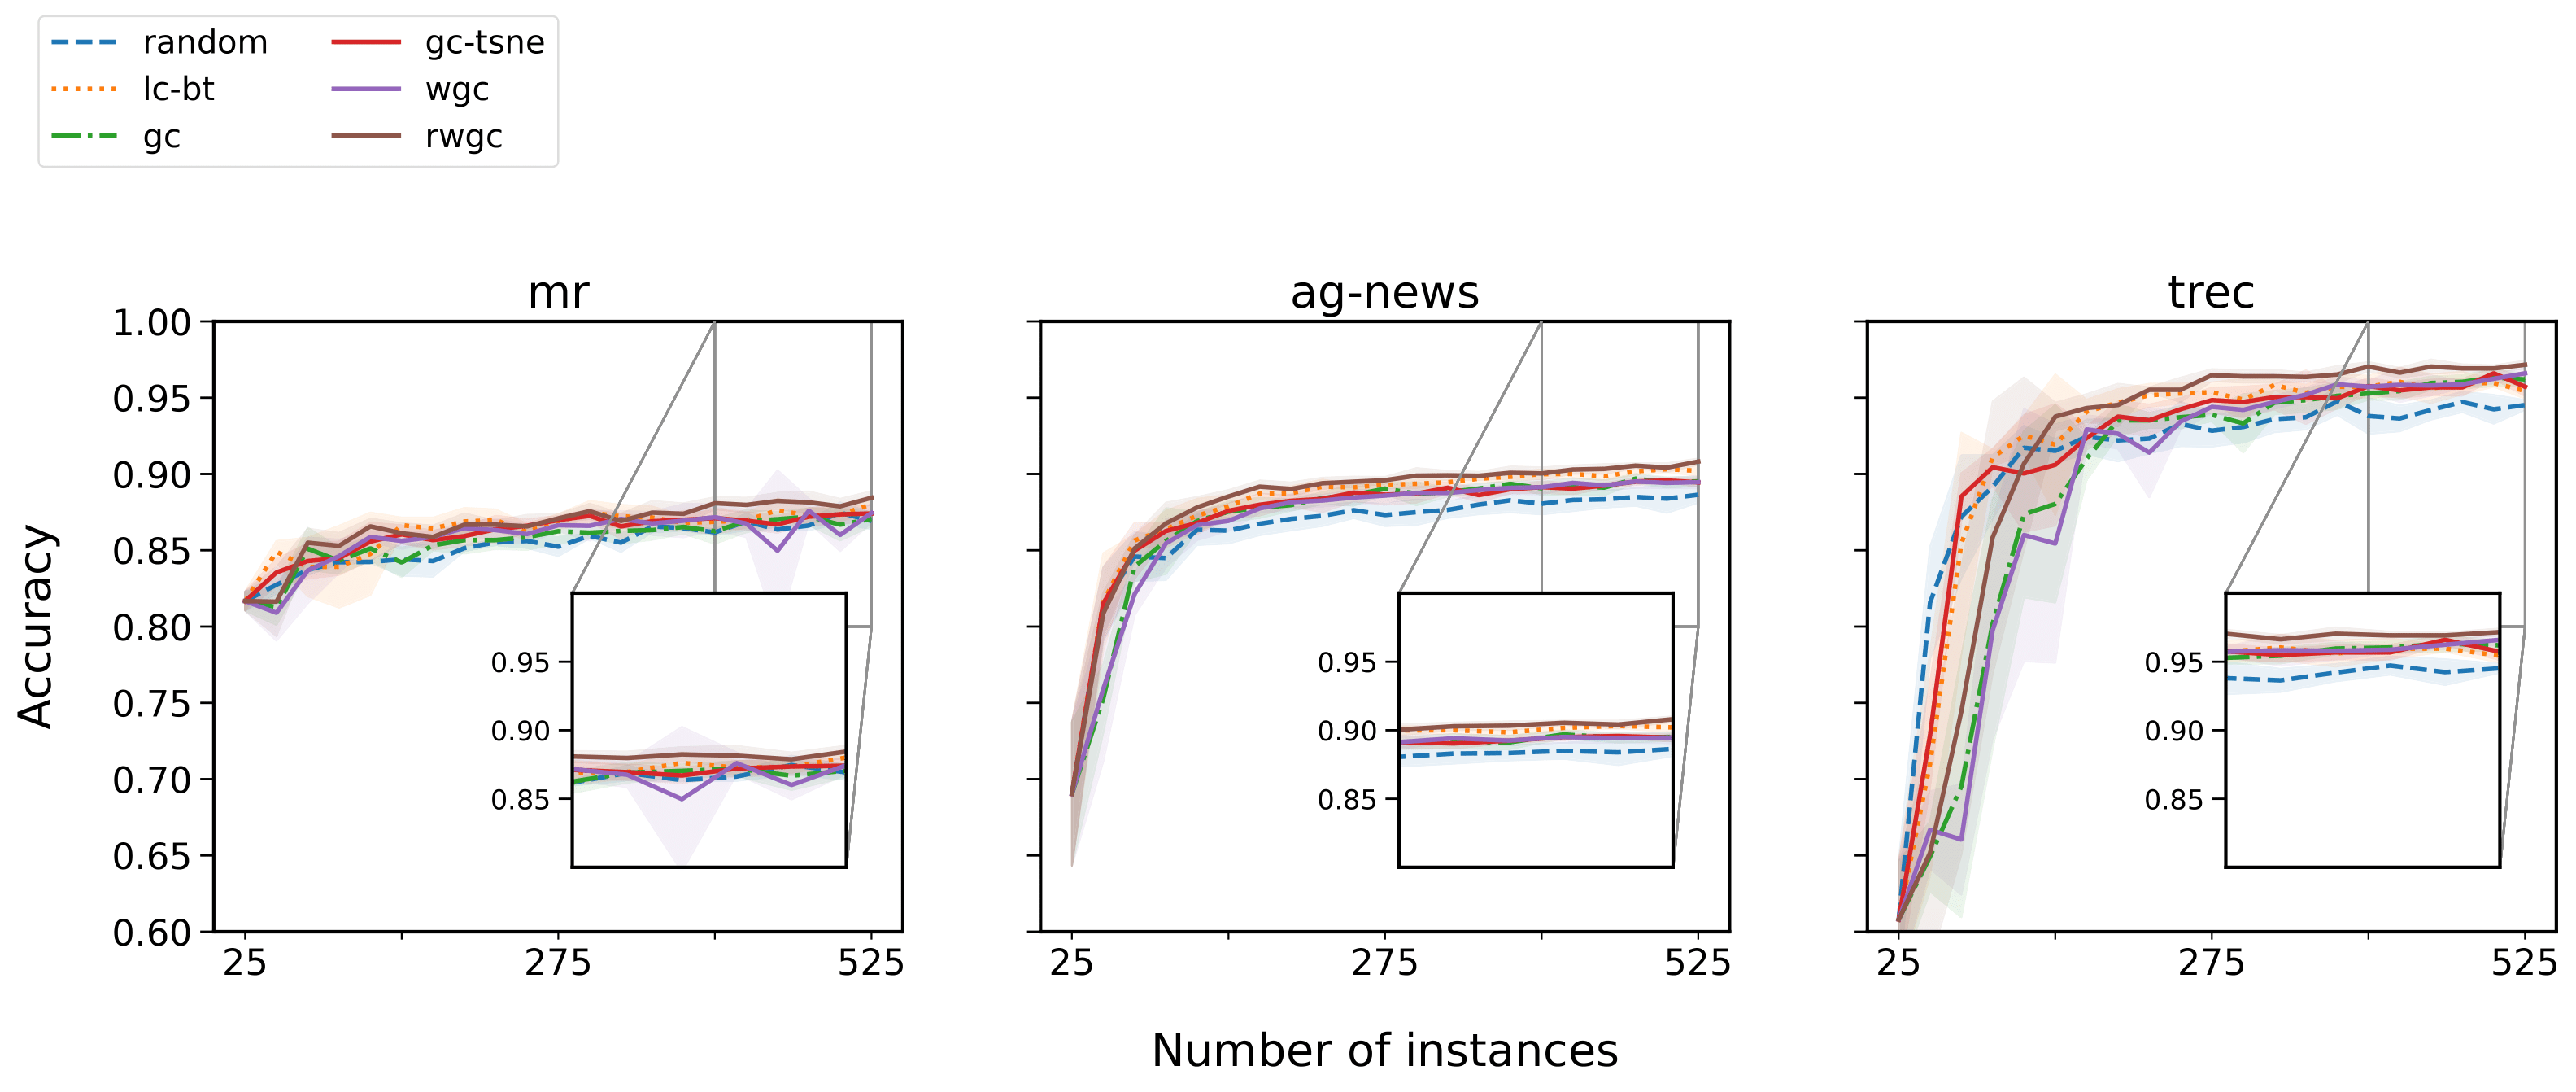
\includegraphics[width=1\textwidth]{img/setfit-plots-1.png}
    \caption{Active Learning curves of SetFit on each dataset when combined with six query strategies: Random Sampling (RS), Breaking-Ties (BT), Greedy Core-Set (CS), Greedy Core-Set with t-SNE (CS-TSNE), Weighted Greedy Core-Set (WCS), and Ranked Weighted Greedy Core-Set (RWCS). The line represents the mean accuracy and the surrounding tubes represent the standard deviation over five runs.}
    \label{fig:setfit-curves}
\end{figure}

\iffalse
%% TEMPLATE TABLE
\begin{table*}[h!]%
\centering
\fontsize{8pt}{9pt}\selectfont%
\renewcommand{\tabcolsep}{12pt}%
\begin{tabular}{@{}ll@{\hspace{10pt}} r @{${}\pm{}$} r r @{${}\pm{}$} r r @{${}\pm{}$} r r @{${}\pm{}$} r @{}}
\toprule
\textbf{Dataset} & \textbf{Model} & \multicolumn{8}{c}{\textbf{Query Strategy}}\\
\cmidrule{3-10} & & \multicolumn{2}{c}{\hspace*{-6pt}RS} & \multicolumn{2}{c}{BT} & \multicolumn{2}{c}{CS} & \multicolumn{2}{c}{\hspace*{4pt}Unknown}\\
\midrule
\multirow{2}{*}{AGN}  & BERT & 1.852 & 0.415 & 0.907 & 0.203 & \bfseries 0.432 & \bfseries 0.097 & 516.554 & 115.583 \\
 & SetFit & 7.264 & 1.626 & \bfseries 6.199 & \bfseries 1.389 & 10.256 & 2.359 & 481.758 & 142.013 \\
\midrule
\multirow{2}{*}{MR}  & BERT & 0.014 & 0.003 & 0.014 & 0.003 & \bfseries 0.009 & \bfseries 0.002 & 1.889 & 0.425\\
 & SetFit & 0.521 & 0.117 & \bfseries 0.436 & \bfseries 0.098 & 0.468 & 0.105 & 3.672 & 1.098 \\
\midrule
\multirow{2}{*}{TREC-6}  & BERT & 0.085 & 0.019 & 0.042 & 0.009 & \bfseries 0.018 & \bfseries 0.004 & 0.609 & 0.138 \\
 & SetFit & 0.289 & 0.065 & \bfseries 0.248 & \bfseries 0.055 & 1.111 & 0.745 & 1.504 & 0.447 \\
\bottomrule
\end{tabular}
\caption{%
Final accuracy per dataset, model, and query strategy. We report the mean and standard deviation over five runs. The best result per dataset is printed in bold.}
\label{table-results-acc}
\end{table*}
\fi

% MY ACC TABLE
\begin{table*}[h!]%
\centering
\fontsize{8pt}{9pt}\selectfont%
\renewcommand{\tabcolsep}{4pt}%
\begin{tabular}{@{}ll@{\hspace{10pt}} r @{${}\pm{}$} r r @{${}\pm{}$} r r @{${}\pm{}$} r r @{${}\pm{}$} r r @{${}\pm{}$} r r @{${}\pm{}$} r @{}}
\toprule
\textbf{Dataset} & \textbf{Model} & \multicolumn{8}{c}{\textbf{Query Strategy}}\\
\cmidrule{3-14} & & \multicolumn{2}{c}{\hspace*{-6pt}RS} & \multicolumn{2}{c}{BT} & \multicolumn{2}{c}{CS} & \multicolumn{2}{c}{\hspace*{4pt}CS-TSNE} & \multicolumn{2}{c}{\hspace*{4pt}WCS} & \multicolumn{2}{c}{\hspace*{4pt}RCS}\\
\midrule

\multirow{2}{*}{AGN}  & BERT & 0.884 & 0.004 & \bfseries 0.889 & \bfseries 0.010 &  0.874 & 0.012 & 0.881 & 0.010 & 0.873 & 0.011 & 0.873 & 0.022\\ 
 & SetFit & 0.886 & 0.006 & 0.902 & 0.004 & 0.895 & 0.003 & 0.895 & 0.003 & 0.895 & 0.005 & \bfseries 0.908 & \bfseries 0.002 \\
 
\midrule
 
\multirow{2}{*}{MR}  & BERT & 0.806 & 0.011 & 0.815 & 0.009 & 0.77 & 0.015 & 0.796 & 0.020 & 0.806 & 0.014 & \bfseries 0.817 & \bfseries 0.010\\ 
 & SetFit & 0.869 & 0.006 & 0.88 & 0.005 & 0.871 & 0.005 & 0.874 & 0.005 & 0.874 & 0.007 & \bfseries 0.884 & \bfseries 0.005 \\

\midrule

\multirow{2}{*}{TREC}  & BERT & 0.904 & 0.018 & 0.92 & 0.014 &  0.902 & 0.021 & 0.912 & 0.009 & 0.897 & 0.027 & \bfseries 0.951 & \bfseries 0.008\\ 
 & SetFit & 0.945 & 0.004 & 0.954 & 0.006 & 0.962 & 0.004 & 0.957 & 0.007 & 0.966 & 0.004 & \bfseries 0.972 & \bfseries 0.003 \\
 
\bottomrule
\end{tabular}
\caption{%
Final accuracy per dataset, model, and query strategy. We report the mean and standard deviation over five runs. The best result per dataset is printed in bold.}
\label{table-results-acc}
\end{table*}

% MY AUC TABLE
\begin{table*}[!t]%
\centering
\fontsize{8pt}{9pt}\selectfont%
\renewcommand{\tabcolsep}{4pt}%
\begin{tabular}{@{}ll@{\hspace{10pt}} r @{${}\pm{}$} r r @{${}\pm{}$} r r @{${}\pm{}$} r r @{${}\pm{}$} r r @{${}\pm{}$} r r @{${}\pm{}$} r @{}}
\toprule
\textbf{Dataset} & \textbf{Model} & \multicolumn{8}{c}{\textbf{Query Strategy}}\\
\cmidrule{3-14} & & \multicolumn{2}{c}{\hspace*{-6pt}RS} & \multicolumn{2}{c}{BT} & \multicolumn{2}{c}{CS} & \multicolumn{2}{c}{\hspace*{4pt}CS-TSNE} & \multicolumn{2}{c}{\hspace*{4pt}WCS} & \multicolumn{2}{c}{\hspace*{4pt}RCS}\\
\midrule

\multirow{2}{*}{AGN}  & BERT & 0.790 & 0.015 & 0.800 & 0.009 & 0.735 & 0.020 & 0.792 & 0.007 & 0.731 & 0.014 & \bfseries 0.805 & \bfseries 0.010\\ 
 & SetFit & 0.865 & 0.007 & 0.881 & 0.004 & 0.871 & 0.005 & 0.875 & 0.004 & 0.87 & 0.003 & \bfseries 0.884 & \bfseries 0.002 \\

\midrule

\multirow{2}{*}{MR}  & BERT & 0.750 & 0.007 & 0.746 & 0.011 & 0.718 & 0.009 & 0.741 & 0.017 & 0.720 & 0.004 & \bfseries 0.759 & \bfseries 0.007\\ 
 & SetFit & 0.854 & 0.002 & 0.864 & 0.005 & 0.856 & 0.003 & 0.862 & 0.003 & 0.858 & 0.007 & \bfseries 0.866 & \bfseries 0.003 \\

\midrule

\multirow{2}{*}{TREC}  & BERT & 0.674 & 0.029 & 0.709 & 0.008 & 0.594 & 0.022 & 0.676 & 0.037 & 0.629 & 0.024 & \bfseries 0.771 & \bfseries 0.021\\ 
 & SetFit & 0.914 & 0.011 & \bfseries 0.923 & \bfseries 0.007 & 0.896 & 0.015 & 0.919 & 0.005 & 0.893 & 0.012 & 0.918 & 0.015 \\
 
\bottomrule
\end{tabular}
\caption{Final AUC per dataset, model, and query strategy. We report the mean and standard deviation over five runs. The best result per dataset is printed in bold.}
\label{table-results-auc}
\end{table*}

The SetFit learning curves generally outperform the BERT model and seem to show much less variation between the different query strategies. When looking at the query strategies, we can see that specifically in the case of BERT, Core-Set seems to underperform especially in earlier iterations, even when compared to RS. This further reinforces the sentiment that Core-Set has its weaknesses when considering the task of text classification. We can see that in most cases, the three variations of Core-Set seem to be on par with or more performant than the original Core-Set. Even so, BT looks to be a strong contender in all cases and manages to perform similarly or better than CS-TSNE and WCS. The largest difference can be seen on the TREC-6 dataset, with RWCS outperforming all other strategies.

In \ref{table-results-acc}, I show the reported mean accuracy and standard deviation for each combination of dataset, model and query strategy. The results show small improvements in accuracy for the dimensionality reduction approach, as well as Weighted Core-Set. However, the Ranked-Weighted Core-Set approach achieves the highest accuracy in almost all instances, being outperformed only on the AG-News dataset with BERT by the Breaking-Ties strategy.

\ref{table-results-auc} contains the reported mean AUC (area under curve) and standard deviation for each combination of dataset, model and query strategy. The top performing AUC results, similarly to the accuracy table, show RWCS as having the best results in almost all cases. 

As also made evident by the learning curves earlier, the accuracy and AUC improvements are most drastic in the case of BERT on the TREC dataset, where RWCS achieves an improvement in Core-Set's mean accuracy of 4.9 percent, and an improvement in AUC of 17.7 percent.

\chapter{Discussion}

\dots

\chapter{Conclusion}

\dots

% \chapter*{Acknowledgements} % optional
% I thank the authors of the webisthesis template for their excellent work!

% \listoffigures % optional, usually not needed

% \listoftables % optional, usually not needed

% \listofalgorithms % optional, usually not needed
%    requires package algorithm2e

% optional: list of symbols/notation (e.g., using the nomencl package) but usually not needed

%\include{chapter1}
%\include{chapter2}

%\include{appendixA}

% Bibliography
\bibliographystyle{plainnat} % requires package natbib. An alternative is apalike
\bibliography{literature}    % load file literature.bib

\end{document}
